\documentclass[12pt, a4paper, oneside]{ctexart}
\usepackage{amsmath, amsthm, amssymb, bm, color, graphicx, geometry, mathrsfs,extarrows, braket, booktabs, array, xcolor, fontspec, appendix, float, subfigure, wrapfig, enumitem, caption}
\usepackage[colorlinks,linkcolor=red,anchorcolor=blue,citecolor=blue,urlcolor=blue,menucolor=black]{hyperref}

%%%% 设置中文字体 %%%%
\setCJKmainfont{方正新书宋_GBK.ttf}[BoldFont = 方正小标宋_GBK, ItalicFont = 方正楷体_GBK, BoldItalicFont = 方正粗楷简体]
%%%% 设置英文字体 %%%%
\setmainfont{Times New Roman}
\setsansfont{Calibri}
\setmonofont{Consolas}

%%%% 设置代码块 %%%%
% 在vscode中使用minted需要先配置python解释器, Ctrl+Shift+P, 输入Python: Select Interpreter选择安装了Pygments的Python版本. 再在setting.json中xelatex和pdflatex的参数中加入 "--shell-escape", 即可
% TeXworks中配置方法参考: https://blog.csdn.net/RobertChenGuangzhi/article/details/108140093
\usepackage{minted}
\renewcommand{\theFancyVerbLine}{
    \sffamily\textcolor[rgb]{0.5,0.5,0.5}{\scriptsize\arabic{FancyVerbLine}}} % 修改代码前序号大小
% 加入不同语言的代码块
\newmintinline{cpp}{fontsize=\small, linenos, breaklines, frame=lines}
\newminted{cpp}{fontsize=\small, linenos, breaklines, frame=lines}
\newmintedfile{cpp}{fontsize=\small, linenos, breaklines, frame=lines}
\newmintinline{matlab}{fontsize=\small, linenos, breaklines, frame=lines}
\newminted{matlab}{fontsize=\small, mathescape, linenos, breaklines, frame=lines}
\newmintedfile{matlab}{fontsize=\small, linenos, breaklines, frame=lines}
\newmintinline{python}{fontsize=\small, linenos, breaklines, frame=lines, python3}  % 使用\pythoninline{代码}
\newminted{python}{fontsize=\small, linenos, breaklines, frame=lines, python3}  % 使用\begin{pythoncode}代码\end{pythoncode}
\newmintedfile{python}{fontsize=\small, linenos, breaklines, frame=lines, python3}  % 使用\pythonfile{代码地址}

%%%% 设置行间距, 页边距, 段落间距 %%%%
\linespread{1.2}
\geometry{left=2.5cm, right=2.5cm, top=2.5cm, bottom=2.5cm}
\newcommand{\setParDis}{\setlength {\parskip} {0.3cm} }

%%%% 定理类环境的定义 %%%%
\newtheorem{example}{例}            % 整体编号
\newtheorem{theorem}{定理}[section] % 定理按section编号
\newtheorem{definition}{定义}
\newtheorem{axiom}{公理}
\newtheorem{property}{性质}
\newtheorem{proposition}{命题}
\newtheorem{lemma}{引理}
\newtheorem{corollary}{推论}
\newtheorem{condition}{条件}
\newtheorem{conclusion}{结论}
\newtheorem{assumption}{假设}
\numberwithin{equation}{section}  % 公式按section编号 (公式右端的小括号)
\newtheorem{algorithm}{算法}

%%%% 自定义环境 %%%%
\newsavebox{\nameinfo}
\newenvironment{myTitle}[1]{
    \begin{center}
    {\zihao{-2}\bf #1\\}
    \zihao{-4}\it
}{\end{center}}  % \begin{myTitle}{标题内容}作者信息\end{myTitle}
\newcounter{problem}  % 问题序号计数器
\newenvironment{problem}[1][]{\stepcounter{problem}\par\noindent\textbf{题目\arabic{problem}. #1}}{\smallskip\par}
\newenvironment{solution}[1][]{\par\noindent\textbf{#1解答. }}{\smallskip\par}  % 可带一个参数表示题号\begin{solution}{题号}
\newenvironment{note}{\par\noindent\textbf{注记. }}{\smallskip\par}
\newenvironment{remark}{\begin{enumerate}[label=\textbf{注\arabic*.}]}{\end{enumerate}}
\BeforeBeginEnvironment{minted}{\vspace{-0.5cm}}  % 缩小minted环境距上文间距
\AfterEndEnvironment{minted}{\vspace{-0.2cm}}  % 缩小minted环境距下文间距

%%%% 图片相对路径 %%%%
\graphicspath{{figure/}} % 当前目录下的figure文件夹, {../figure/}则是父目录的figure文件夹
\setlength{\abovecaptionskip}{-0.2cm}  % 缩紧图片标题与图片之间的距离
\setlength{\belowcaptionskip}{0pt} 

%%%% 缩小item,enumerate,description两行间间距 %%%%
\setenumerate[1]{itemsep=0pt,partopsep=0pt,parsep=\parskip,topsep=5pt}
\setitemize[1]{itemsep=0pt,partopsep=0pt,parsep=\parskip,topsep=5pt}
\setdescription{itemsep=0pt,partopsep=0pt,parsep=\parskip,topsep=5pt}

%%%% 自定义公式 %%%%
\everymath{\displaystyle} % 默认全部行间公式, 想要变回行内公式使用\textstyle
\DeclareMathOperator*\uplim{\overline{lim}}     % 定义上极限 \uplim_{}
\DeclareMathOperator*\lowlim{\underline{lim}}   % 定义下极限 \lowlim_{}
\DeclareMathOperator*{\argmax}{arg\,max}  % 定义取最大值的参数 \argmax_{}
\DeclareMathOperator*{\argmin}{arg\,min}  % 定义取最小值的参数 \argmin_{}
\let\leq=\leqslant % 简写小于等于\leq (将全部leq变为leqslant)
\let\geq=\geqslant % 简写大于等于\geq (将全部geq变为geqslant)
\DeclareRobustCommand{\rchi}{{\mathpalette\irchi\relax}}
\newcommand{\irchi}[2]{\raisebox{\depth}{$#1\chi$}} % 使用\rchi将\chi居中

%%%% 一些宏定义 %%%%
\def\bd{\boldsymbol}        % 加粗(向量) boldsymbol
\def\disp{\displaystyle}    % 使用行间公式 displaystyle(默认)
\def\tsty{\textstyle}       % 使用行内公式 textstyle
\def\sign{\text{sign}}      % sign function
\def\wtd{\widetilde}        % 宽波浪线 widetilde
\def\R{\mathbb{R}}          % Real number
\def\N{\mathbb{N}}          % Natural number
\def\Z{\mathbb{Z}}          % Integer number
\def\Q{\mathbb{Q}}          % Rational number
\def\C{\mathbb{C}}          % Complex number
\def\K{\mathbb{K}}          % Number Field
\def\P{\mathbb{P}}          % Polynomial
\def\d{\mathrm{d}}          % differential operator
\def\e{\mathrm{e}}          % Euler's number
\def\i{\mathrm{i}}          % imaginary number
\def\re{\mathrm{Re}}        % Real part
\def\im{\mathrm{Im}}        % Imaginary part
\def\res{\mathrm{Res}}      % Residue
\def\ker{\mathrm{Ker}}      % Kernel
\def\vspan{\mathrm{vspan}}  % Span  \span与latex内核代码冲突改为\vspan
\def\L{\mathcal{L}}         % Loss function
\def\wdh{\widehat}          % 宽帽子 widehat
\def\ol{\overline}          % 上横线 overline
\def\ul{\underline}         % 下横线 underline
\def\add{\vspace{1ex}}      % 增加行间距
\def\del{\vspace{-1.5ex}}   % 减少行间距

%%%% 正文开始 %%%%
\begin{document}

%%%% 定义标题页,包括title,author,affiliation,email等 %%%%
\title{NLP大作业报告\\基于Bert的中文商品评论分类模型}
\author{
西安交通大学,数学与统计学院,强基数学\\[3ex]
吴天阳$^a$,马煜璇$^b$,孙思雨$^c$,陈江河$^d$\\[1ex]
2204210460$^a$,2204220461$^b$,2206124483$^c$, 2204411197$^d$\\[2ex]
}
\date{\today}
\maketitle % 设置上面的标题
\clearpage % 创建新的一面
\tableofcontents % 创建目录页,使用目录需要编译两次, 并且不能删去编译产生的临时文件!!!

\clearpage
\section{实验目的}
使用GitHub上商品评论的\href{https://github.com/SophonPlus/ChineseNlpCorpus/blob/master/datasets/online_shopping_10_cats/intro.ipynb}{数据集},总共10个商品类别,包含两种情绪,总计$62773$条数据. 正向评论:$31727$条,负向评论:$31046$条.

使用Bert预训练模型,对每条评论进行词向量转换,输出层连接一个有$11$个神经元的全连接神经网络对文本进行分类.

调整超参数,包括:不同的预处理序列长度,优化器的选择,输出层前神经网络的层数. 自定义验证数据,验证模型的泛化性.
\section{实验原理}
Bert模型原理参考文章:

\begin{enumerate}
\def\labelenumi{\arabic{enumi}.}
\item
  \href{https://cloud.tencent.com/developer/article/1389555}{图解BERT模型:从零开始构建BERT}
  这篇文章详细的介绍了Bert的原理、transformer模型和Attention机制.
  (以下图片均来自该博客)
\item
  \href{https://zhuanlan.zhihu.com/p/98855346}{什么是BERT?}
  这两篇文章都介绍了Bert模型的输入输出还有Bert的结构,第二篇更简短一些.
  其预训练部分使用的原理,MLM和NSP过程,不用很具体的讲解,只需要大致介绍他们俩分别起到什么功能.
\end{enumerate}

Bert模型是一种\textbf{无监督学习的预训练模型}(能进行迁移学习的模型,用于各种NLP问题),模型主要就是将transformer模型进行堆叠而形成的,其输入与输出的维度相同,过程类似于词编码过程,将低维的词向量进行编码,并将其特征进行放大,与其他特征进行分离.
\subsection{模型结构}

NLP,BERT,Transformer,Attention之间的关系,如图\ref{fig-relation}所示.

\begin{figure}[htbp]
\centering
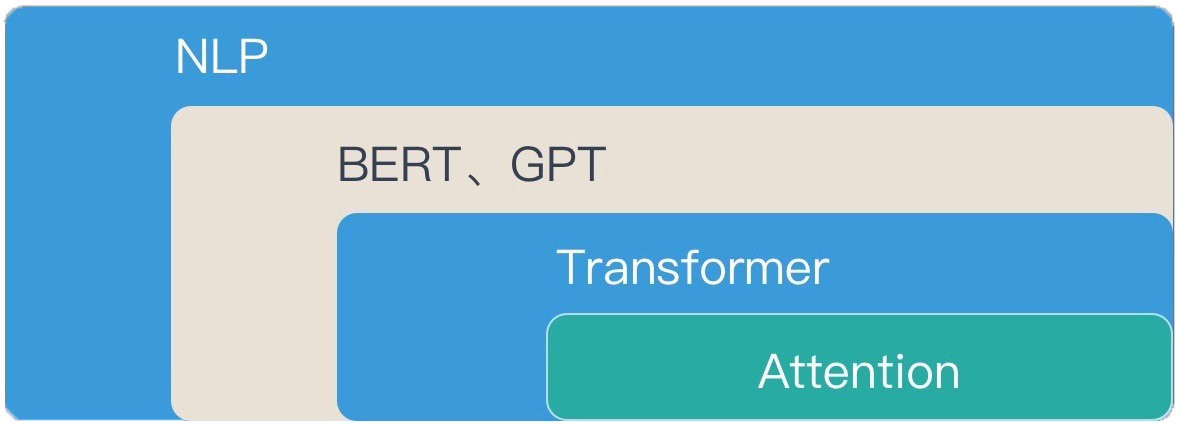
\includegraphics[scale=0.4]{../NLP大作业note.figure/Bert,Transformer,Attention之间的关系.jpg}
\caption{NLP模型之间的关系}
\label{fig-relation}
\end{figure}

\subsubsection{Attention机制}

Attention机制主要思路就是:\textbf{通过机器学习得到单词之间的权重分布,然后作用在特征上}.

Attention机制有三种实现方式:RNN+Attention,CNN+Attention,纯Attention,第三种就是Google团队在2017发表的论文\href{https://arxiv.org/pdf/1706.03762.pdf}{Attention
is All you need}中提到的,上述模型都是使用该思路搭建的.

\begin{wrapfigure}[15]{r}{.5\linewidth} % 文字环绕行数为13行, 图片靠右 (l为靠左), 图片占0.5的行宽
    \centering
    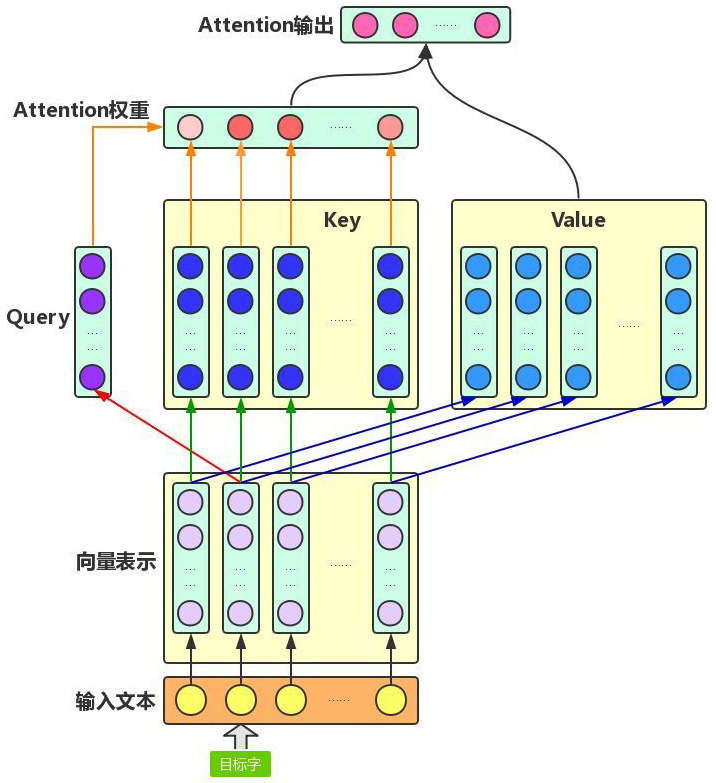
\includegraphics[scale=0.4]{../NLP大作业note.figure/Attention机制.jpg}
    \caption{Attention机制}
    \label{fig-attention}
\end{wrapfigure}
这里以单个文字的Attention权重计算为例,首先将该句话总每个文字使用神经网络转化为向量表示形式(词向量),取定一个文字作为当前的Query目标,将上下文的文字作为Key,并同时另存到Value值内.
然后计算Query值和Key值的相关性(利用内积进行计算),并通过softmax函数得到Attention权重(归一化),最后再对Value向量使用Attention权重加权求和,即可得到Attention机制后的输出. 如图\ref{fig-attention}所示.

我们再对该句话中每一个文字都进行如上操作即可得到整句话的Attention输出,由于只融合了该句话字之间的相关性,所以也称为Self-Attention,如图\ref{fig-self-attention}所示.

\vspace{2cm}
\begin{figure}[htbp]
    \centering
    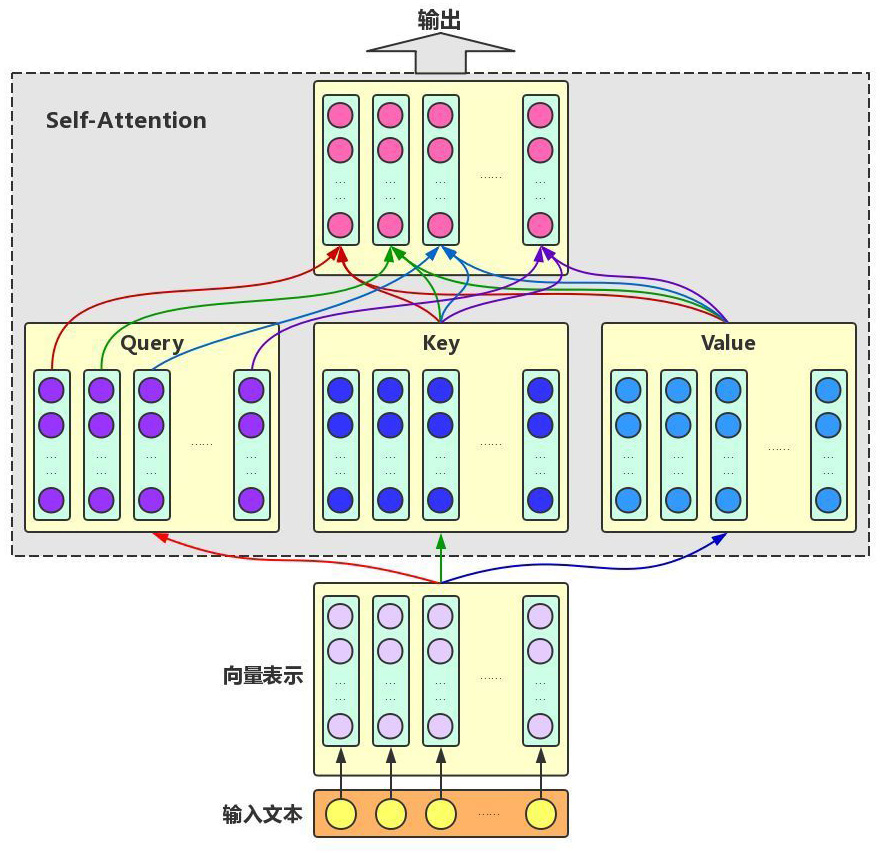
\includegraphics[scale=0.4]{../NLP大作业note.figure/Self-Attention.png}
    \caption{Self-Attention模型}
    \label{fig-self-attention}
\end{figure}

\clearpage
\begin{wrapfigure}[11]{l}{.7\linewidth}
\centering
\hspace{-3cm}
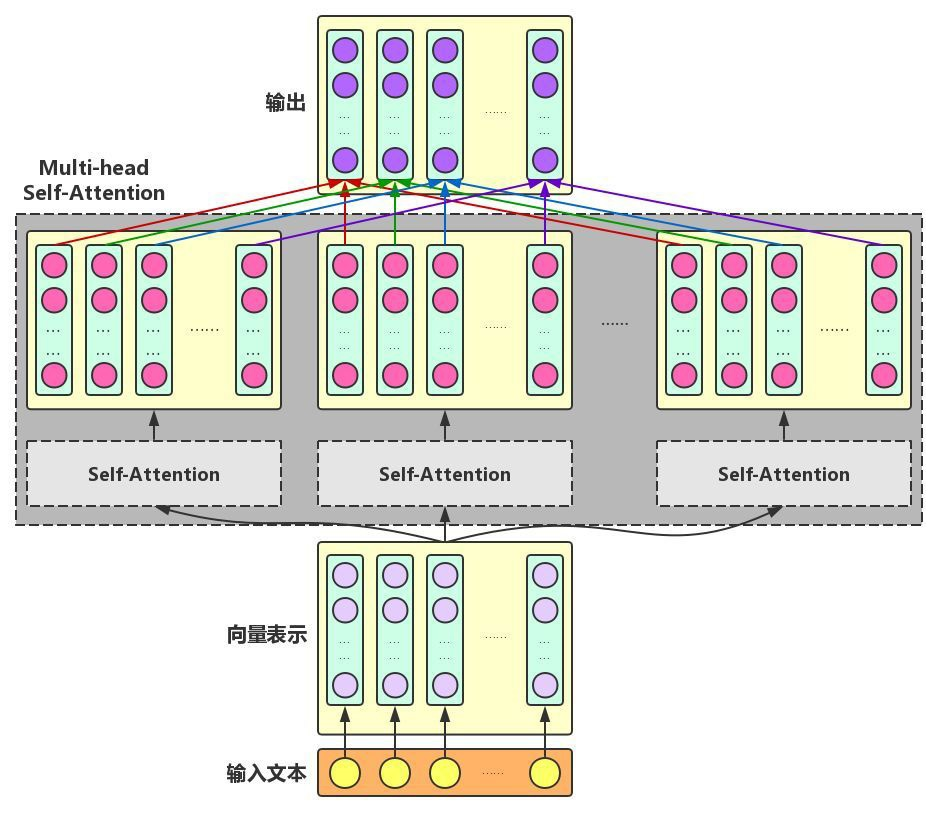
\includegraphics[scale=0.4]{../NLP大作业note.figure/Multi-head Self-Attention.jpg}
\captionsetup{justification=raggedright, singlelinecheck=false}
\caption{Multi-head-Self-Attention}
\label{fig-multi-head-self-attention}
\end{wrapfigure}
为了进一步提高Attention处理的多样性,处理不同语义空间下的增强向量,Multi-head Self-Attention模型中进一步叠加Self-Attention,最后连接神经网络保持输出层和原始向量长度相同,这就得到了Multi-head Self-Attention,如图\ref{fig-multi-head-self-attention}所示.

\vspace{1.5cm}
\begin{wrapfigure}[15]{r}{.6\linewidth}
\centering
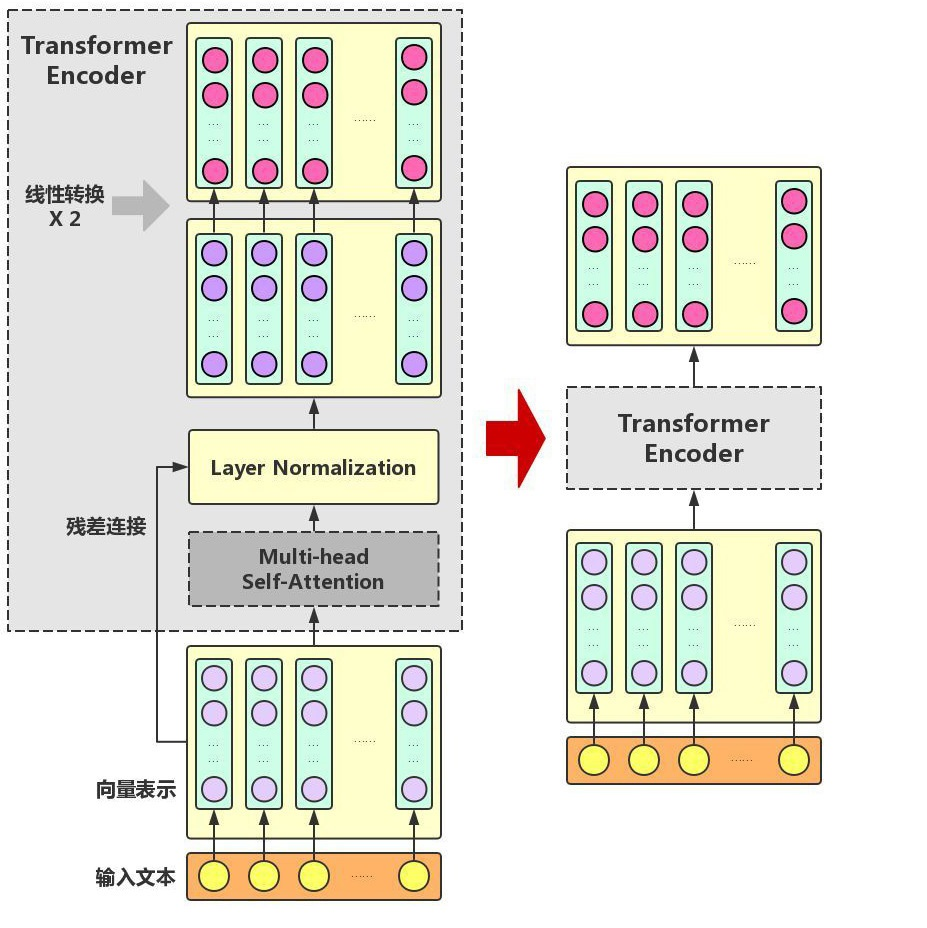
\includegraphics[scale=0.4]{../NLP大作业note.figure/Transformer.jpg}
\caption{Transformer模型}
\label{fig-transformer}
\end{wrapfigure}
\ \vspace{3.5cm}

\subsubsection{Transformer Encoder}
由于Berd中只是用了Transformer的编码部分,所以只对其进行介绍.
Transformer主要是在Multi-head Self-Attention的基础上加入了三个操作(模型如图\ref{fig-transformer}所示):
1. 残差连接(Residual Connection):此处使用的思路应该是来自2015年ImageNet图像识别比赛第一名的\href{https://arxiv.org/abs/1512.03385}{ResNet},其主要用于解决深度神经网络在深度过高之后数据过度离散的问题,主要解决了过多的非线性函数导致网络难以实现恒等变换的问题,同样该操作使得网络变得更加容易训练.

2. 层标准化(Layer Normalization):对某一层神经网络做均值为0方差为1的标准化操作,主要为了避免网络过深导致loss值过小的问题.

3. 两次线性变换:两层神经网络处理,增强模型的表达能力(保持输入与输出长度相同).
\clearpage
{
\begin{wrapfigure}[20]{r}{.4\linewidth}
\centering
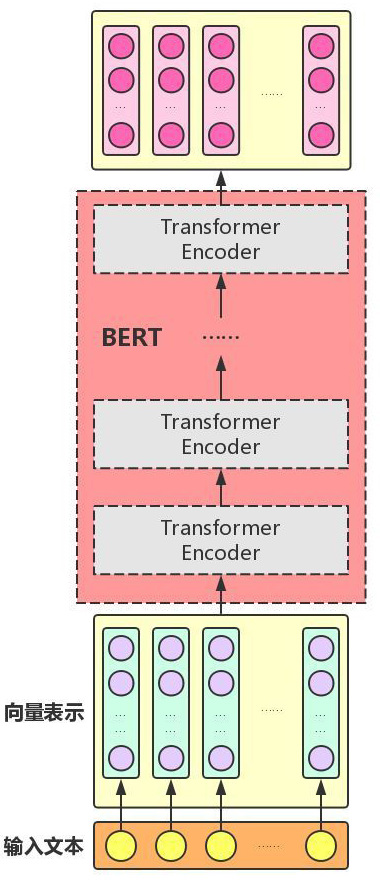
\includegraphics[scale=0.4]{../NLP大作业note.figure/Bert.jpg}
\caption{Bert模型}
\label{fig-bert}
\end{wrapfigure}
\subsubsection{Bert模型}

在Transformer模型基础上对其进行堆叠,最后连接全连接神经网络降低特征维数,这样就完成了Bert模型基本框架,模型如图\ref{fig-bert}所示.(论文中使用的堆叠层数为12层和24层,我们将使用12层的Bert模型进行训练)

\subsection{预训练任务}

有了Bert模型之后,为了使该模型具有泛化能力,能够用于处理各种NLP问题,论文作者以Wiki作为数据集对模型进行预训练(如同在读懂文章之前,学会如何理解句式,学习语言的本身).
Bert模型主要由以下两个预训练模型构成:

1. Masked Language Model(MLM),在一句话中随机掩去该句话中的几个字,通过剩余的字去预测掩去的字是什么,类似英文中的完形填空,本质是在模仿人类学习语言的方法,这样的好处在于迫使机器去依赖上下文预测词汇,增强上下文词汇之间的关联性,并赋予其一定的纠错能力. 如图\ref{fig-MLM}所示.

}
\begin{wrapfigure}[8]{l}{.5\linewidth}
\centering
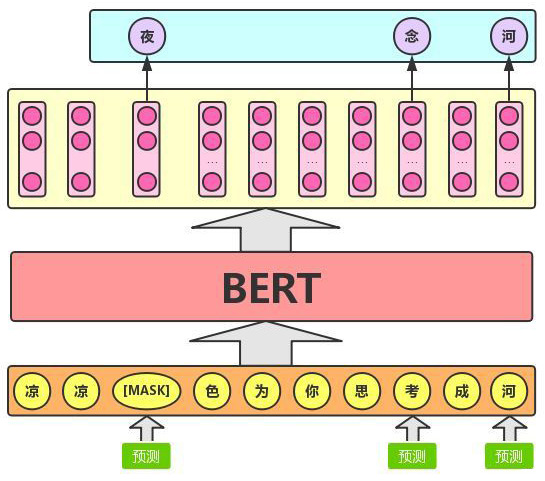
\includegraphics[scale=0.4]{../NLP大作业note.figure/Masked Language Model.jpg}
%\captionsetup{justification=raggedright, singlelinecheck=false}
\caption{MLM任务}
\label{fig-MLM}
\end{wrapfigure}
\ \vspace{0.5cm}

2. Next Sentence Prediction(NSP):通过给出文章中的两句话,判断第一句话是否出现在第二句话之后,类似高中语文的古诗词默写和英文的段落重排,该训练可以使模型学习到整篇文章内容之间的关联性,更准确的刻画语句之间的信息. 如图\ref{fig-NSP}所示.

\vspace{2.5cm}
\subsection{模型应用}
对于不同的现实场景Bert模型通过构建不同的输出层维度从而完成不同的分类问题,例如:单文本分类(通过在文章的开头加入{[}CLS{]}符号表示文章的语义信息),语义场景分类(使用{[}SEP{]}分隔符作为两句话之间的分隔),序列标注问题等等,参考图\ref{fig-NSP}中的输入部分. (在程序设计中的预处理部分会详细解释)

更一般的,可以通过对Bert模型的输出进行微调从而完成各种分类问题,即对编码后的向量连接全连接神经网络到输出层,对模型进行训练.

\begin{figure}[htbp]
\centering
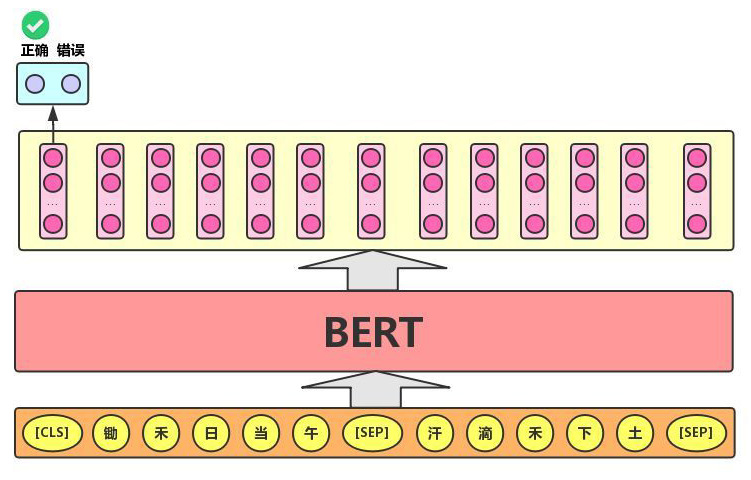
\includegraphics[scale=0.4]{../NLP大作业note.figure/Next Sentence Prediction part1.png}
\caption{NSP任务}
\label{fig-NSP}
\end{figure}

\vspace{-0.3cm}
\section{实验步骤与结果分析}
试验所使用的Python环境为3.9.15,神经网络框架为TensorFlow2.9.1及以上版本,使用Bert模型必备库为\pythoninline{tensorflow_hub, tensorflow_text}(使用pip安装对应TensorFlow版本的即可),其他常用库为\pythoninline{numpy, pandas, matplotlib, tqdm}.
\subsection{数据处理}
使用\pythoninline{pandas}库做数据处理部分,首先删去评论中的无效数据项
\begin{pythoncode}
df = pd.read_csv(data_handle)  # 数据读入
df = df[df.review.isna() == False]  # 删去Nan项
\end{pythoncode}
对数据类别进行编号,构造从类别空间到$\Z^{10}$的双射
\begin{pythoncode}
class2idx = {}  # 从类别到编号的映射
idx2class = {}  # 从编号到类别的映射
for idx, name in enumerate(class_names):
    class2idx[name] = idx
    idx2class[idx] = name
\end{pythoncode}
不同类别的正负样例数目不同,如下表所示
\renewcommand\arraystretch{0.8} % 设置表格高度为原来的0.8倍
\begin{table}[!htbp] % table标准
    \hspace{-0.8cm}
    \begin{tabular}{p{1.4cm}<{\centering}p{1cm}<{\centering}p{1cm}<{\centering}p{1cm}<{\centering}p{1cm}<{\centering}p{1.4cm}<{\centering}p{1.4cm}<{\centering}p{1cm}<{\centering}p{1cm}<{\centering}p{1.4cm}<{\centering}p{1cm}<{\centering}} % 设置表格宽度
        \toprule
类别  & 书籍   & 平板    & 手机   & 水果    & 洗发水   & 热水器 & 蒙牛   & 衣服    & 计算机  & 酒店    \\
        \midrule
总数目 & 3851 & 10000 & 2323 & 10000 & 10000 & 574 & 2033 & 10000 & 3992 & 10000 \\
正例  & 2100 & 5000  & 1165 & 5000  & 5000  & 474 & 992  & 5000  & 1996 & 5000  \\
负例  & 1751 & 5000  & 1158 & 5000  & 5000  & 100 & 1041 & 5000  & 1996 & 5000 \\
        \bottomrule
    \end{tabular}
\end{table}

首先将每种类别商品的数据按照3:1划分为训练集和验证集,然后对训练集进行补全到$7500$个数据,正负样例分别为$3750$个,若不足,则随机选取补齐.
\begin{pythoncode}
train_ds, val_ds = None, None  # 训练集与验证集
for name in class_names:
    tmp = df[df.cat==name]
    pos_num, neg_num = tmp[tmp.label==1].shape[0], tmp[tmp.label==0].shape[0]  # 获取当前类别下正例与负例数目
    pos_ds = tf.data.Dataset.from_tensor_slices((tmp[tmp.label==1]['review'], [(1, class2idx[name]) for _ in range(pos_num)]))  # 正例集合
    neg_ds = tf.data.Dataset.from_tensor_slices((tmp[tmp.label==0]['review'], [(0, class2idx[name]) for _ in range(neg_num)]))  # 负例集合
    
    pos_num = pos_num * val_split // 100  # 划分给验证集的正例数目
    neg_num = neg_num * val_split // 100  # 划分给验证集的负例数目
    pos_val = pos_ds.take(pos_num)  # 正例验证集
    pos_train = pos_ds.skip(pos_num)  # 正例训练集
    neg_val = neg_ds.take(neg_num)  # 负例验证集
    neg_train = neg_ds.skip(neg_num)  # 负例训练集
    
    train_marge = pos_train.concatenate(neg_train).shuffle(10000, seed=seed).repeat(-1)  # 合并正负数据,再补齐到7500个数据
    train_ds = train_marge.take(7500) if train_ds is None else train_ds.concatenate(train_marge.take(7500))  # 合并训练集
    val_ds = pos_val.concatenate(neg_val) if val_ds is None else val_ds.concatenate(pos_val).concatenate(neg_val)  # 合并验证集
\end{pythoncode}
\vspace{-0.5cm}
\subsection{模型搭建}
Bert模型被分为两部分:\pythoninline{Bert_preprocessor, Bert_encoder},前者对输入特征进行预处理操作,加入[CLS]符号与[SEP]符号,进行mask操作与段落分段任务的标记(对应MLM和NSP任务);后者是Bert模型的主要部分,包括12个Transformer块和最后输出的全连接神经网络. 下面我们详细分析每一部分的具体实现方法.
\subsubsection{预处理模型}
模型来自\href{https://tfhub.dev/tensorflow/bert_zh_preprocess/3}{TF-hub: bert\_zh\_preprocess},对句子的预处理的输出包括三个部分:
\begin{enumerate}
  \item \pythoninline{input_mask}:二进制掩码,$1$表示模型可以知道该处的字,$0$表示模型无法知道该处的字.(用于MLM任务)
  \item \pythoninline{input_word_ids}:将每个字进行编码,其中\pythoninline{101}表示[CLS],\pythoninline{102}表示[SEP].
  \item \pythoninline{input_type_ids}:只有在有两句话判断上下文时有用,用于告诉模型两句话的位置. 第一段$0$表示第一句话,第一段$1$表示第二句话.(用于NSP任务)
\end{enumerate}
模型搭建部分如下,\pythoninline{seq_length}为自定义转化的最大字符串长度.
\begin{pythoncode}
# preprocessor_handle为预加载模型的本地路径,或者为官网下载链接
def bert_preprocessor(sentence_features, seq_length=128):
    text_inputs = [layers.Input(shape=(), dtype=tf.string, name=ft)
                   for ft in sentence_features]  # 设定文本的输入
    
    preprocessor = hub.load(preprocessor_handle)  # 加载预处理模型
    # tokenize可以将每个句子划分为单个的字
    tokenize = hub.KerasLayer(preprocessor.tokenize, name='tokenizer')
    tokenized_inputs = [tokenize(segment) for segment in text_inputs]  

    # packer加载预处理模型中将tokenize结果进一步打包输出为上述三种形式
    packer = hub.KerasLayer(
        preprocessor.bert_pack_inputs,
        arguments=dict(seq_length=seq_length),
        name='packer'
    )
    encoder_inputs = packer(tokenized_inputs)
    return keras.Model(text_inputs, encoder_inputs, name='preprocessor')
preprocessor = bert_preprocessor(['input1'])  # 构建一个输入句子的预处理模型
\end{pythoncode}
对于输入的字符串\pythoninline{"你好 "},预处理部分会在字符串的开头和结尾处加上开始符号[CLS]和分隔符号[SEP],转化为\pythoninline{"[CLS]你好[SEP]"},从而在原有序列长度上增加$2$.

下面我们对其进行验证(\pythoninline{101,102}分别表示[CLS],[SEP]):
\begin{pythoncode}
x = tf.constant(['你好呀', '不好但是'])
x_preprocessed = preprocessor(x)
print(f"{'Keys':<15}: {list(x_preprocessed.keys())}")
print(f"{'Shape Word Ids':<15}: {x_preprocessed['input_word_ids'].shape}")
print(f"{'Word Ids':<15}: {x_preprocessed['input_word_ids'][0,:12]}")
print(f"{'Shape Mask':<15}: {x_preprocessed['input_mask'].shape}")
print(f"{'Input Mask':<15}: {x_preprocessed['input_mask'][0,:12]}")
print(f"{'Shape Type Ids':<15}: {x_preprocessed['input_type_ids'].shape}")
print(f"{'Type Ids':<15}: {x_preprocessed['input_type_ids'][0,:12]}")
""" 输出结果
Keys           : ['input_mask', 'input_word_ids', 'input_type_ids']
Shape Word Ids : (2, 128)
Word Ids       : [101 872 1962 1435 102  0  0  0  0  0  0  0]
Shape Mask     : (2, 128)
Input Mask     : [1 1 1 1 1 0 0 0 0 0 0 0]
Shape Type Ids : (2, 128)
Type Ids       : [0 0 0 0 0 0 0 0 0 0 0 0]
"""
\end{pythoncode}
使用\pythoninline{tf.keras.utils.plot_model}api输出模型的架构图,如图\ref{fig-preprocessor}所示.
\begin{figure}[htbp]
  \centering
  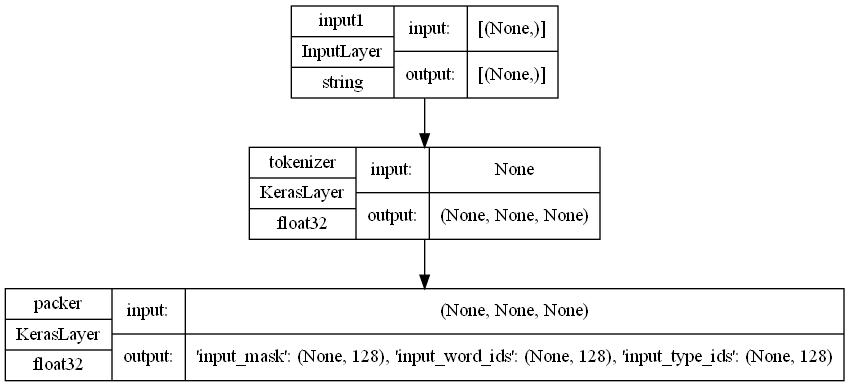
\includegraphics[scale=0.5]{Preprocessor.png}
  \setlength{\abovecaptionskip}{0cm}
  \caption{Preprocessor模型}
  \label{fig-preprocessor}
\end{figure}

\subsubsection{Bert分类模型}
已预训练的Bert编码模型来自\href{https://tfhub.dev/tensorflow/bert_zh_L-12_H-768_A-12/4}{TF-hub: bert\_zh\_L-12\_H-768\_A-12},从模型论文\href{https://arxiv.org/pdf/1810.04805.pdf}{BERT: Pre-training of Deep Bidirectional Transformers for Language Understanding
}中可知,模型编号中L为Transformer块个数,H为隐藏层大小(输出维度),A为每个Transormer中Self-Attention的个数. 

Bert编码模型的输出包含三个部分:
\begin{enumerate}
  \item \pythoninline{pooled_output}:输出的特征向量,最后经过全连接层后输出的结果,大小为$768$维.
  \item \pythoninline{sequence_output}:最后一个Transformer块的输出结果,大小为\pythoninline{[128, 768]}维.
  \item \pythoninline{encoder_outputs}:大小为$12$的list,包含Transformer块的输出结果.
\end{enumerate}
我们要用汇聚后的输出特征\pythoninline{pooled_output},连接一层0.3抛弃率的\pythoninline{Dropout}层,最后通过两个全连接神经网络,其中一个包含1个神经元作为情感分类,另一个包含2个神经元作为商品分类. 模型搭建代码如下
\begin{pythoncode}
# encoder_handle为Bert模型的本地路径,或者为官网下载链接
def build_classifier():
    text_input = layers.Input(shape=(), dtype=tf.string, name='input')
    text_preprocessed = preprocessor(text_input)  # 使用已搭建的预处理模型
    encoder = hub.KerasLayer(encoder_handle, trainable=True, name='BERT_encoder')  # 导入Bert模型
    x = encoder(text_preprocessed)['pooled_output']
    x = layers.Dropout(0.3)(x)
    x1 = layers.Dense(1, name='emotion')(x)
    x2 = layers.Dense(10, name='classifier')(x)
    return keras.Model(text_input, [x1, x2])
classifier_model = build_classifier()
\end{pythoncode}
还是使用\pythoninline{tf.keras.utils.plot_model}显示模型框架,如图\ref{fig-bert-encoder}所示
\begin{figure}[htbp]
  \centering
  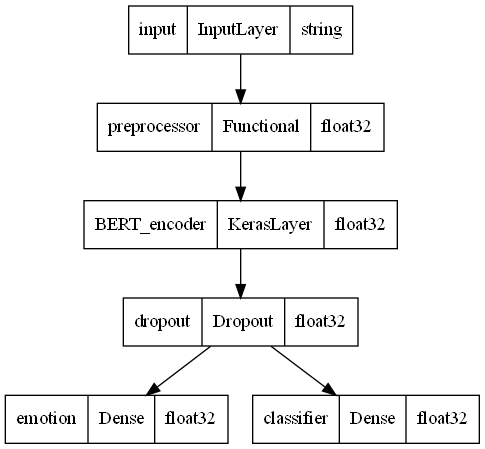
\includegraphics[scale=0.5]{Bert_encoder.png}
  \setlength{\abovecaptionskip}{0cm}
  \caption{基于Bert编码的分类模型}
  \label{fig-bert-encoder}
\end{figure}
\subsection{模型训练与验证}
下面进行超参数配置和设置模型参数记录器:
\begin{pythoncode}
# 超参数配置
batch_size = 32
batch_N = 100000 / batch_size
epochs = 1
lr_change = None  # 根据epoch训练个数动态调整步长
optimizer = optimizers.Adam(learning_rate=1e-4)  # Adam优化器,设定步长
binary_loss = losses.BinaryCrossentropy(from_logits=True)  # 损失函数
multi_loss = losses.SparseCategoricalCrossentropy(from_logits=True)
# 随机打乱样本,设定batch大小
dataset = ds.shuffle(100000).batch(batch_size).repeat(epochs)

# 情感分类上的准确率
emotion_acc = keras.metrics.BinaryAccuracy('emotion_acc')
# 情感分类上的平均损失
emotion_loss= keras.metrics.Mean('emotion_loss', dtype=tf.float32)
# 物品分类上的准确率
class_acc = keras.metrics.SparseCategoricalAccuracy('class_acc')
# 物品分类上的平均损失
class_loss = keras.metrics.Mean('class_loss', dtype=tf.float32)
metrics = [emotion_acc, emotion_loss, class_acc, class_loss]
\end{pythoncode}
下面为训练与验证部分的核心代码,验证与训练的主要差别是无需计算梯度,并将模型训练关闭\pythoninline{training=False},这样才不会启用Dropout操作.
\begin{pythoncode}
def test(val_ds):  # 模型测试
    for (x, y) in val_ds:
        emotion_y = tf.reshape(y[:, 0], [-1, 1])  # 情感标签
        classes_y = tf.reshape(y[:, 1], [-1, 1])  # 分类标签
        emotion, classes = classifier_model(x, training=False)
        loss1 = binary_loss(emotion_y, emotion)
        loss2 = multi_loss(classes_y, classes)

        emotion_acc.update_state(emotion_y, emotion)
        emotion_loss.update_state(loss1)
        class_acc.update_state(classes_y, classes)
        class_loss.update_state(loss2)

def train():  # 模型训练
    global optimizer  # 为了能修改全局变量
    for step, (x, y) in tqdm(enumerate(train_ds)):
        emotion_y = tf.reshape(y[:, 0], [-1, 1])  # 情感标签
        classes_y = tf.reshape(y[:, 1], [-1, 1])  # 分类标签
        with tf.GradientTape() as tape:
            emotion, classes = classifier_model(x, training=True)  # 预测
            loss1 = binary_loss(emotion_y, emotion)  # y=(batch, 2)
            loss2 = multi_loss(classes_y, classes)
            loss = tf.reduce_mean(loss1 + loss2)  # 将loss求和作为总损失
        grads = tape.gradient(loss, classifier_model.trainable_variables)
        optimizer.apply_gradients(zip(grads, classifier_model.trainable_variables))  # 更新网络参数

        emotion_acc.update_state(emotion_y, emotion)
        emotion_loss.update_state(loss1)
        class_acc.update_state(classes_y, classes)
        class_loss.update_state(loss2)

        if step % 100 == 0:
            save_metrics()  # 保存计数器结果
            metrics.reset_states()  # 重置计数器
            test(val_ds.take(100))  # 仅验证100*batch_size个数据
            draw_figure()  # 绘制结果图
            classifier_model.save_weights(ckp_save_handle)  # 保存模型权重
            print(f"Save in '{ckp_save_handle}'")

        if lr_change is not None and step == batch_N:  # 调整步长
            optimizer = optimizers.Adam(learning_rate=lr_change[step//batch_N])
            print("调整步长为", lr_change[step//batch_N])
\end{pythoncode}
模型训练参数变化图如下图所示(epochs=1, Dropout=0.3,Seqlength=128):
\begin{figure}[htbp]
    \hspace{-2.5cm}
    \subfigure  % 子图的标题
    {
        % 如果一行放三个图改成0.3\linewidth即可
        \begin{minipage}[b]{.62\linewidth}
            \centering
            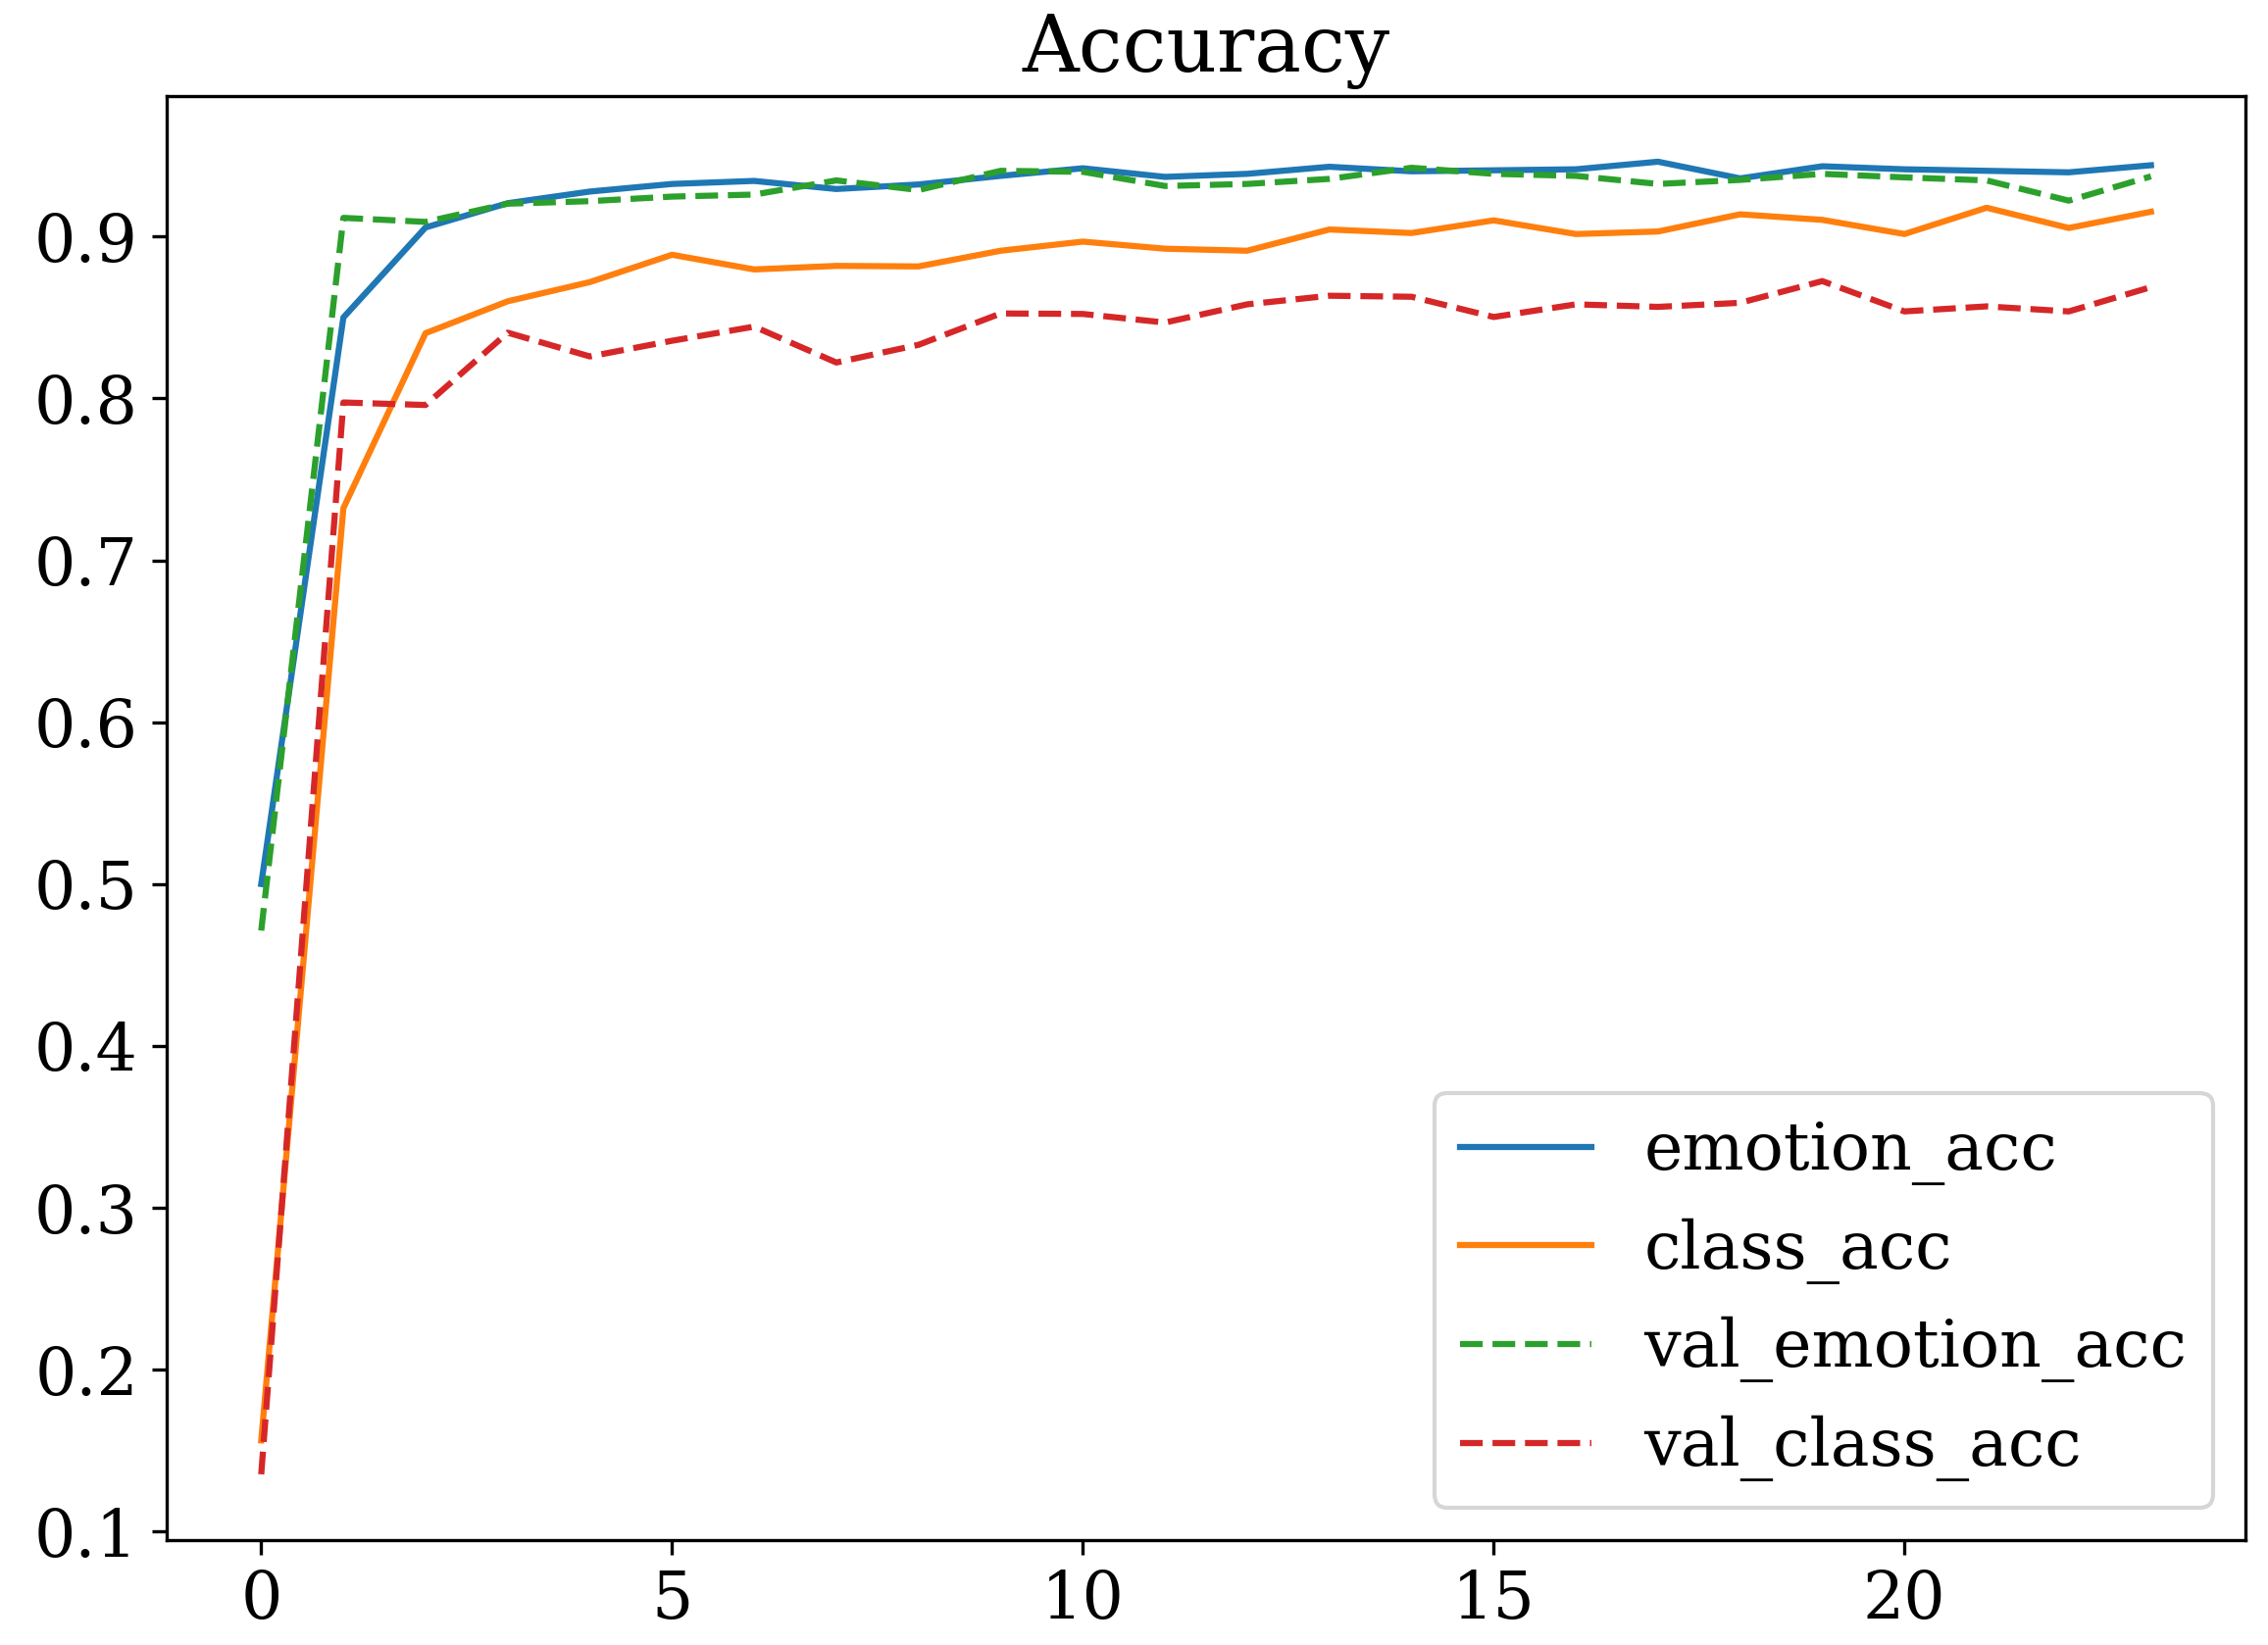
\includegraphics[scale=0.5]{acc_dropout0.1.png}
        \end{minipage}
    }
    \subfigure
    {
        \begin{minipage}[b]{.2\linewidth}
            \centering
            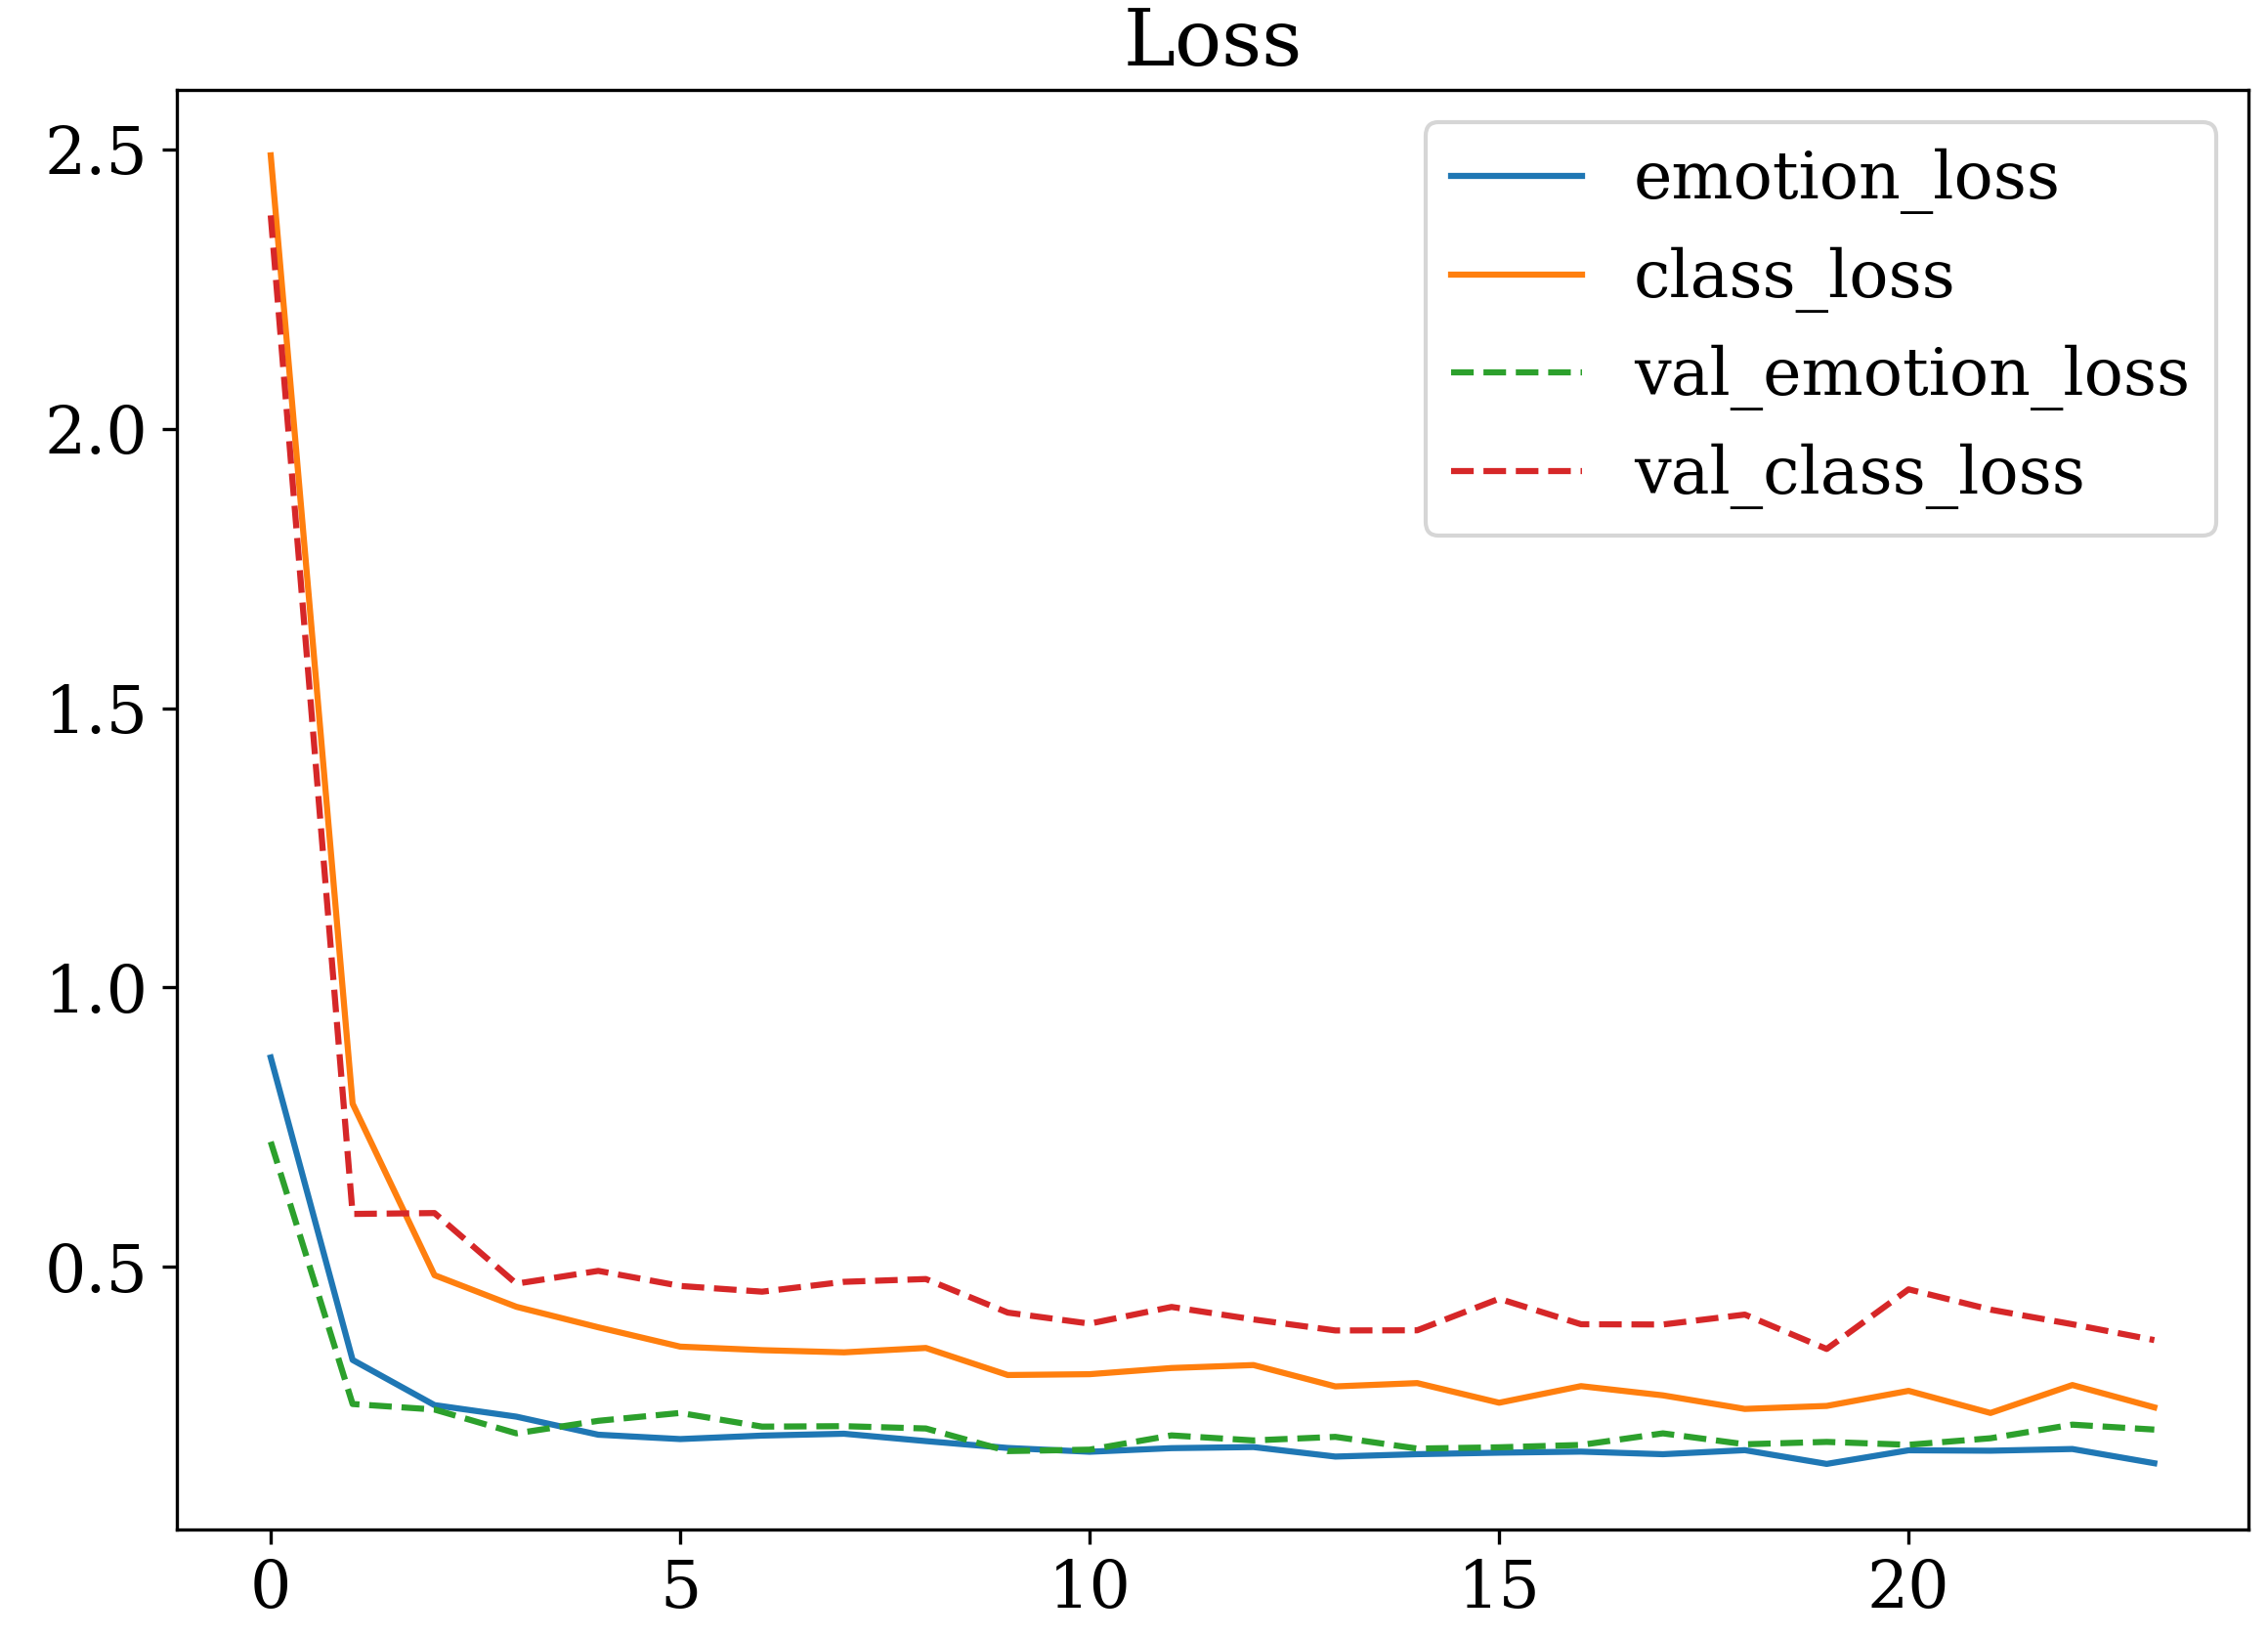
\includegraphics[scale=0.5]{loss_dropout0.1.png}
        \end{minipage}
    }
\end{figure}
\vspace{-1cm}
\subsubsection{网络模型调整}
我们尝试修改了输出端的网络参数,得到了以下的训练结果:(epoch=2, 在第一个epoch时使用$10^{-4}$的步长, 在第二个epoch时使用$10^{-5}$的步长)

1. batch=32, Dropout=0.3, Seqlength=128:
\begin{pythoncode}
emotion_acc=0.978 emotion_loss=0.070 class_acc=0.952 class_loss=0.130
验证集上情感分类准确率: 94.57%
验证集上商品分类准确率: 90.63%
\end{pythoncode}

2. batch=32, Dropout=0.1, Seqlength=128:
\begin{pythoncode}
emotion_acc=0.966 emotion_loss=0.095 class_acc=0.948 class_loss=0.146
验证集上情感分类准确率: 93.99%
验证集上商品分类准确率: 90.59%
\end{pythoncode}

3. batch=16, Dropout=0.3, Seqlength=256:
\begin{pythoncode}
emotion_acc=0.957 emotion_loss=0.114 class_acc=0.940 class_loss=0.164
验证集上情感分类准确率: 93.26%
验证集上商品分类准确率: 89.45% 
\end{pythoncode}

测试自定义评论可以使用如下方法
\begin{pythoncode}
def binary_classifier(out):
    ret = []
    for item in out:
        ret.append(1 if item[0] > 0.5 else 0)
    return ret

def multi_classifier(out, num=3):  # 输出前num个的类别
    ret = []
    for item in out:
        classes = []
        arg = np.argsort(item.numpy())[::-1]
        for i in range(num):
            classes.append((idx2class[arg[i]], np.round(item[arg[i]].numpy(), 2)))
        ret.append(classes)
    return ret

x = ["写的稀烂,太差了", "写的真好,期待后续出版", ...]  # 自定义评论
emotion, classes = classifier_model(tf.constant(x), training=False)
emotion = binary_classifier(emotion)  # 转化为正负情感
classes = multi_classifier(classes, num=3)  # 显示排名前三的类别
for i in range(len(x)):
    print(f"\"{x[i]}\":{emotion[i]},{classes[i]}")
"""输出结果
"写的稀烂,太差了":0,[('书籍', 4.02), ('衣服', 3.67), ('酒店', 2.49)]
"写的真好,期待后续出版":1,[('书籍', 3.55), ('平板', 2.44), ('衣服', 2.08)]
"""
\end{pythoncode}
\subsubsection{使用外部数据集作为验证集}
我们打算使用Amazon商品数据集作进一步的验证,\href{https://github.com/SophonPlus/ChineseNlpCorpus/blob/master/datasets/yf_amazon/intro.ipynb}{yf\_amazon数据集下载位置}.

该数据集主要分为三个文件

1. \pythoninline{rating.csv}中存储了用户评论的各种信息,包含评论具体内容与打分,可以通过\pythoninline{productID}找到对应的商品.

2. \pythoninline{products.csv}中存储了每个\pythoninline{productID}对应的商品名称与类别编号\pythoninline{catIds}.

3. \pythoninline{categories.cvs}中存储了每种\pythoninline{catId}对应的类别名称.
\\
使用方法:首先在\pythoninline{categories.cvs}中找到目标类别对应的\pythoninline{catId},然后在\pythoninline{products.csv}中找到包含该种分类编号的商品,最后从\pythoninline{rating.csv}中找到对应的评论. 我们期望将每种类别的文件保存到对应的文件当中.

\begin{pythoncode}
amazon_df = pd.read_csv('../dataset/yf_amazon/ratings.csv')
products_df = pd.read_csv('../dataset/yf_amazon/products.csv')
cats_df = pd.read_csv('../dataset/yf_amazon/categories.csv')
cats = [[832], [642], [304], [-1], [1121], [702], [-1],
        [1100, 965, 903, 899, 875, 717, 585, 569, 534, 331, 245, 90], [1057], [-1]]  # 需要类别名称对应的类别编号
for cat, name in zip(cats, cat_names):
    def check(row):
        items = [int(a) for a in row['catIds'].split(',')]  # 将类别用逗号划分开
        for item in items:
            if item in cat:
                return True
        return False
    products = products_df[products_df.apply(check, axis=1)]['productId']
    item_df = amazon_df[amazon_df.apply(lambda row: row['productId'] in products, axis=1)][['rating', 'comment']]
    print(f"'{name}'类别中商品数目{products.shape[0]},评论数目{item_df.shape[0]}")
    item_df = item_df.sort_values(by=['rating'], ascending=False, ignore_index=True)  # 按评分排序保存到文本中
    item_df.to_csv(f"./validation/{name}.csv", index=False)
\end{pythoncode}

每种类别对应的文件数目如下
\begin{pythoncode}
'书籍'类别中商品数目383500, 评论数目2842292
'平板'类别中商品数目363, 评论数目13341
'手机'类别中商品数目1861, 评论数目81211
'水果'类别中商品数目0, 评论数目0
'洗发水'类别中商品数目501, 评论数目13923
'热水器'类别中商品数目204, 评论数目3853
'蒙牛'类别中商品数目0, 评论数目0
'衣服'类别中商品数目5557, 评论数目2332
'计算机'类别中商品数目20112, 评论数目359804
'酒店'类别中商品数目0, 评论数目0
\end{pythoncode}

我们发现服装数据中的数据有较多的书籍评论,所以将其删去. 由于对于平板和手机的评论十分类似,我们打算用预测结果中前3个中正确则认为预测正确. 预测代码如下所示
\begin{pythoncode}
class_acc = [0, 0]  # 物品分类上的准确率

# 真实值在前num个中则认为正确
def update_acc(classes_y, classes, acc, num=3):
    for b in range(classes.shape[0]):
        acc[1] += 1
        pred = classes[b]
        arg = np.argsort(pred.numpy())[::-1]
        for i in range(num):
            if classes_y[b] == arg[i]:
                acc[0] += 1
                break

for (x, y) in tqdm(val_ds.batch(128)):
    emotion_y = tf.reshape(y[:, 0], [-1, 1])  # 情感标签
    classes_y = tf.reshape(y[:, 1], [-1, 1])  # 分类标签
    emotion, classes = classifier_model(x, training=False)
    emotion_acc.update_state(emotion_y, emotion)
    update_acc(classes_y, classes, class_acc)

print(f"情感分类准确率: {emotion_acc.result().numpy():.2%}")
print(f"商品分类准确率: {class_acc[0]/class_acc[1]:.2%}")
print(f"总计验证数目:{emotion_acc.count.numpy()}")
\end{pythoncode}
最终测试如下三个模型在Amazon验证集上的正确率:\\\pythoninline{bert_classifier_epoch1}参数为batch=32, epochs=1, Seqlength=128;\\
\pythoninline{bert_classifier_epoch2}参数为batch=32, epochs=2, Seqlength=128;\\
\pythoninline{bert_classifier_seq_256}参数为batch=16, epochs=2, Seqlength=256.
\begin{pythoncode}
bert_classifier_epoch1
情感分类准确率: 73.95%
商品分类准确率: 84.04%

bert_classifier_epoch2
情感分类准确率: 78.74%
商品分类准确率: 81.75%

bert_classifier_seq_256
情感分类准确率: 76.38%
商品分类准确率: 83.71%
\end{pythoncode}
\section{结论与讨论}
全部代码均已上传至GitHub仓库:\href{https://github.com/wty-yy/LaTex-Projects/tree/main/NLP/NLP%E5%A4%A7%E4%BD%9C%E4%B8%9A/code}{大作业代码},主要Jupyter代码\href{https://github.com/wty-yy/LaTex-Projects/blob/main/NLP/NLP%E5%A4%A7%E4%BD%9C%E4%B8%9A/code/main.ipynb}{main.ipynb},脚本代码\href{https://github.com/wty-yy/LaTex-Projects/blob/main/NLP/NLP%E5%A4%A7%E4%BD%9C%E4%B8%9A/code/main.py}{main.py},可共部署的代码:\href{https://github.com/wty-yy/Bert-Chinese-Text-Classifier-Tensorflow2}{Bert-Chinese-Text-Classifier-Tensorflow2}.

通过本次实验我们学习了如何使用神经网络进行NLP的分类问题,首先我们学习了Bert的基本原理,与神经网络的编码基础知识;参考官方教程,学会如何使用Bert预训练模型进行文本的编码,对我们要训练的数据进行划分,训练集进行填充平均,使得每种类别的数据均匀分配,并搭建用于实际分类问题的神经网络;我们尝试了不同的输出层的神经网络,调整训练的次数、每次训练使用的步长、预处理文本的最大长度,最终比对不同模型的在验证集下的准确率,并自定义输入数据进行模型检验.

本次大作业提高了我们对复杂模型神经网络模型的训练,学会了数据的各种处理方式,为以后科研打下基础.

%%%% 以下部分是正文 %%%%  
\end{document}
